\documentclass{article} % kind of document 
\usepackage[utf8]{inputenc} %encoding of choice
\usepackage[american]{babel} %language of choice
\usepackage[p,osf]{cochineal}
\usepackage{fancyhdr} %for header
\usepackage{amsmath, tabu} %math mode
\usepackage{mathtools}
\usepackage{extarrows} % for more options with arrows
\usepackage{amssymb} %math symbols
\usepackage{dsfont} %specifically for the indicator function symbol
\usepackage{xcolor} %to color text
\usepackage{amsthm} %math theorem
\usepackage{tikz}
\usepackage{caption}
\usepackage{multirow}
\usepackage[bottom]{footmisc}
% \usepackage[dvipsnames]{xcolor}
\usepackage{enumerate} %make lists
\usepackage{graphicx} %insert images
\usepackage{float} %to fix image position
\usepackage{moreverb} %to make boxes
\usepackage{hyperref} %to create hyperlinks
\usepackage{lipsum} %lorem ipsum package
\usepackage{setspace} % to use singlespace below in the solution environment
\usepackage[shortlabels]{enumitem}
\usepackage{parskip}
\usepackage[us]{datetime} %package for setting due date in US format
\newdate{duedate}{20}{10}{2021} %to set a due date
\allowdisplaybreaks
\usepackage[margin=1in]{geometry}
\pagestyle{fancy}
\usepackage{jlcode}

\lhead{Due: \displaydate{duedate}}
\chead{ECON 899 -- Problem Set 6}
\rhead{Danny, Hiroaki, Mitch, Ryan, Yobin}


\DeclareMathOperator*{\E}{\mathbb{E}} %ease of writing e and E
\newcommand{\e}{\mathrm{e}}
\newcommand{\ct}{\mathsf{c}}
\newcommand{\Z}{\mathbb{Z}}
\newcommand{\R}{\mathbb{R}}
\newcommand{\N}{\mathbb{N}}
\newcommand{\ifn}{\mathds{1}}
\newcommand{\X}{\mathbf{X}}
\newcommand{\Y}{\mathbf{Y}}
\newcommand{\one}{\mathbf{1}}
\newcommand\numberthis{\addtocounter{equation}{1}\tag{\theequation}}
\newcommand*\widebar[1]{\overline{#1}} % to get a widebar
\theoremstyle{definition}
\newtheorem{theorem}{theorem} % Theorem display format
\newtheorem{problem}[theorem]{Exercise} % Problem display format, last bracket sets display choice

\newenvironment{solution}[1][Answer]{\begin{singlespace}\underline{\textbf{#1:}}\quad }{\ \rule{0.3em}{0.3em}\end{singlespace}} % Answer format

\newenvironment{solutions}[1][Proof]{\begin{singlespace}\underline{\textbf{#1:}}\quad }{\ \rule{0.3em}{0.3em}\end{singlespace}} % Answer format

\begin{document}
Tasks:
\subsubsection*{Task 1}
Solve both versions of the model presented above. Use the parameter values in the calibration section of section 1 for both versions.
\begin{solution}
Our code is attached in the appendix.
\end{solution}
\subsubsection*{Task 2}
Compute the following model moments and fill in the table. Are they any different across model specifications? If yes, try to explain intuitively what drives the differences.
\begin{solution}
	The table is the following:
	\begin{center}
	\begin{tabular}{ccccc}
		variable & Standard & TV1 Shock $\alpha$ = 1.0 & TV1 Shock $\alpha$ = 2.0 & TV1 Shock $\alpha$ = 3.0\\
		\hline
		Price Level & 0.739 & 0.713 & 0.725 & 0.728\\
		Mass of Incumbents & 8.32 & 10.336 & 8.83 & 8.216\\
		Mass of Entrants & 2.638 & 2.757 & 3.031 & 3.209\\
		Mass of Exits & 1.662 & 2.133 & 2.132 & 2.087\\
		Aggregate Labor & 185.37 & 191.285 & 183.026 & 178.805\\
		Labor of Incumbents & 142.625 & 152.537 & 142.519 & 137.856\\
		Labor of Entrants & 42.746 & 38.748 & 40.507 & 40.949\\
		Fraction of Labor Entrants & 0.231 & 0.203 & 0.221 & 0.229\\
		\hline
		Average Time In & 4.155 & 4.745 & 3.907 & 3.559\\
		$\int W(s;p)\nu(ds)$ & 3.696 & 3.567 & 3.627 & 3.645\\

	\end{tabular}
	\end{center}

	There are differences across model specifications. As the variance of the TV1 shock increases, the equilibrium price level decreases. This suggests that increasing the TV1 shock variance tends to increase $\int W(s;p)\nu(ds)$ for a given value of $p$. A partial explanation for why could be that conditional on entering, the average number of periods an entrant tends to stay in the market is increasing in the variance of the TV1 shock, as shown in the ``Average Time In'' row. In equilibrium, $\int W(s;p)\nu(ds)$ is decreasing in the variance of the TV1 shock. Since it takes longer for firms to exit the market upon entering, the mass of incumbents at any given time is therefore increasing in the variance of the TV1 shock. This explains the general trend of the ``Mass of Incumbents'' row, and seems also to explain why the mass and labor of entrants respectively shrink relative to the mass and labor of incumbents as the variance of the TV1 shock rises. The ``Mass of Exits,'' ``Aggregate Labor,'' and ``Incumbent Labor'' also tend to rise with the variance of the TV1 shock, which is likely because there is a larger total number of firms in the market at higher values of the TV1 shock variance.
\end{solution}

\subsubsection*{Task 3}
Plot the decision rules of exit in all model specifications you have solved. Are they any different? If yes, try to explain intuitively what drives the differences.
\begin{solution}
Figure \ref{T3} displays the results. There are differences across model specifications.  The benchmark model shows that, absent the shocks, all firms optimally exit the market at a productivity of 3.98e-4 but stay in at all higher productivity levels. Therefore, the only reason a firm would deviate from this plan of action is if they received an appropriate shock, and the larger the variance of the shock, the greater the chances that a firm will deviate. This explains why, as the variance of the TV1 shock increases, the probability of exiting the market decreases when firm productivity is 3.98e-4 and increases when firm productivity is at 3.58.
	\begin{figure}[htbp]
	\begin{center}
	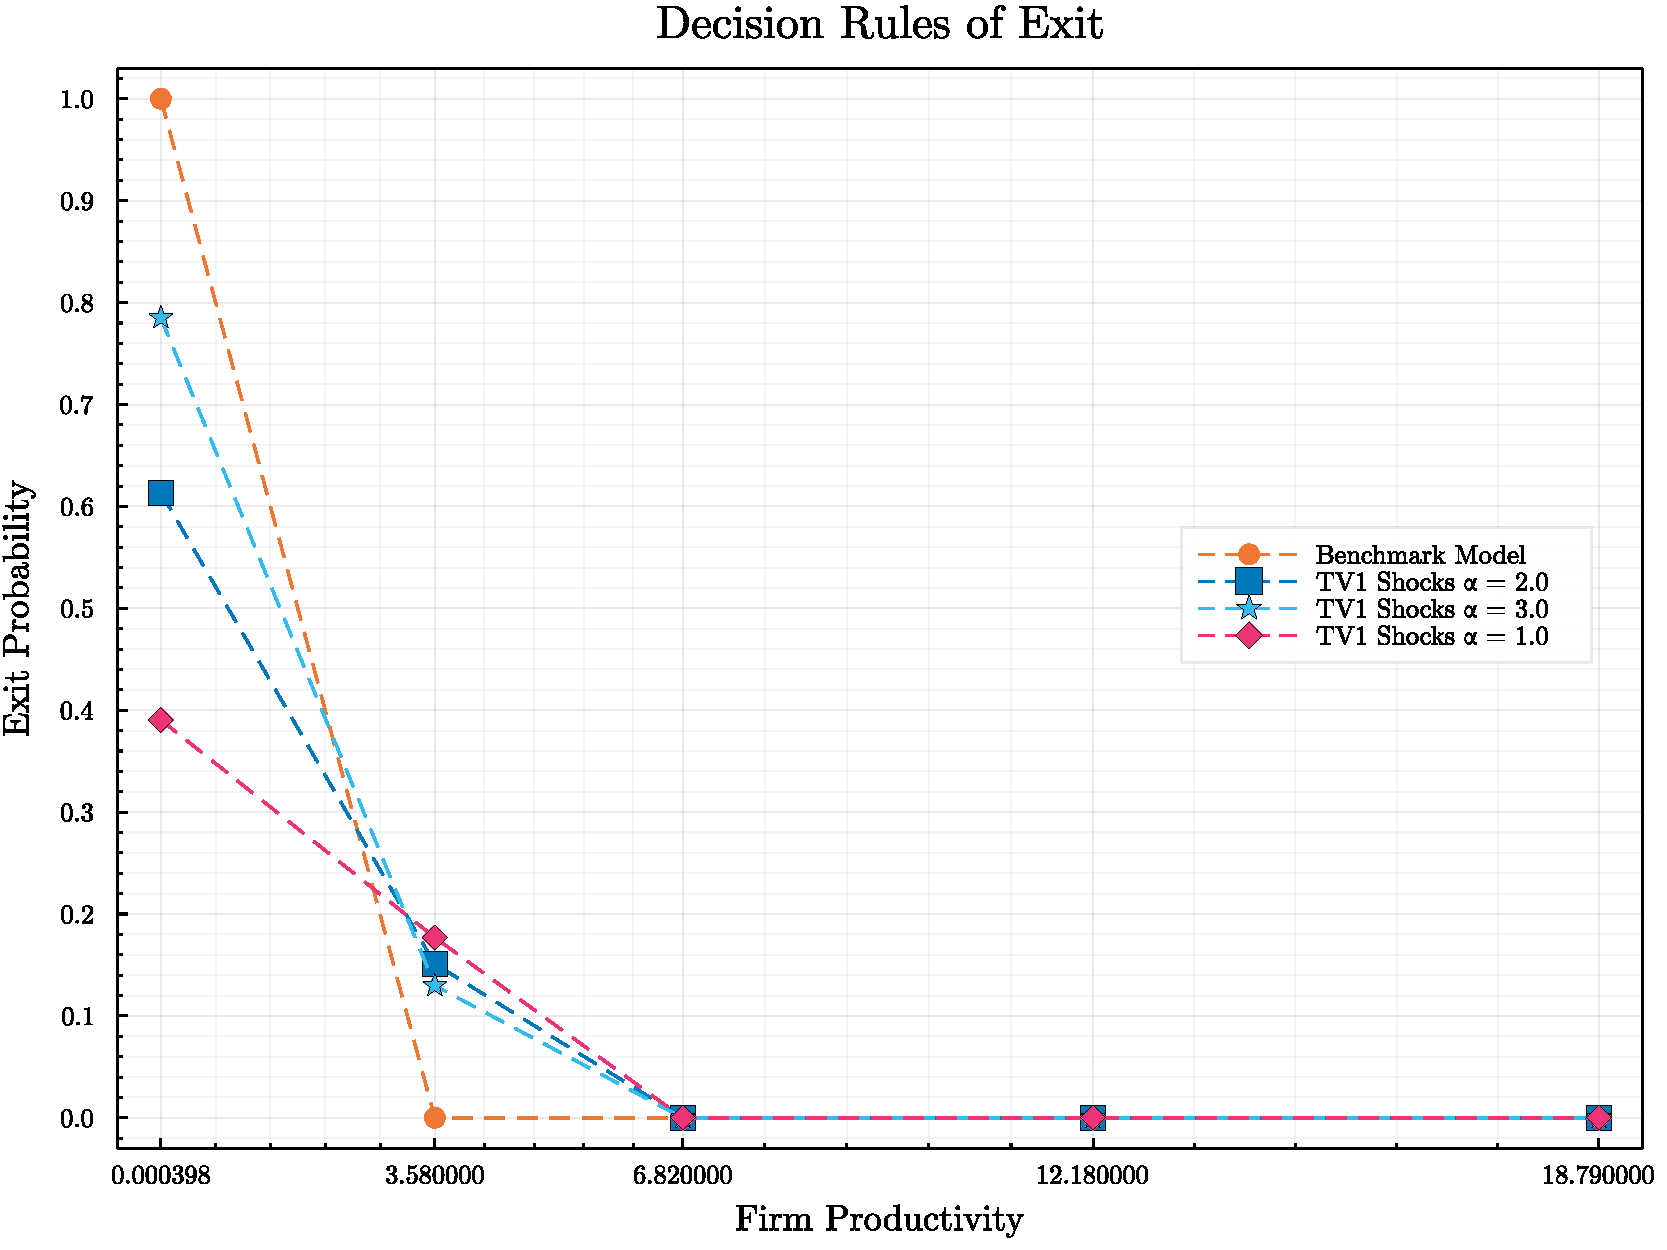
\includegraphics[scale=.35]{Figures/decision_rules.pdf}
	\caption{Decision Rules across Model Specifications}
	\label{T3}
	\end{center}
	\end{figure}
\end{solution}

\subsubsection*{Task 4}
How does the exit decision rule change if cf rises from 10 to 15?

\begin{solution}
Figure \ref{T4} shows the results. Relative to the case shown in figure \ref{T3} where $c_{f}=10$, now under the benchmark model firms optimally exit when their productivity level is at 3.58 as well as when it is at 3.98e-4. When $c_{f}=15$, firms become less likely to exit as the variance of the TV1 shock increases for each of these two productivity levels.
\begin{figure}[htbp]
	\begin{center}
	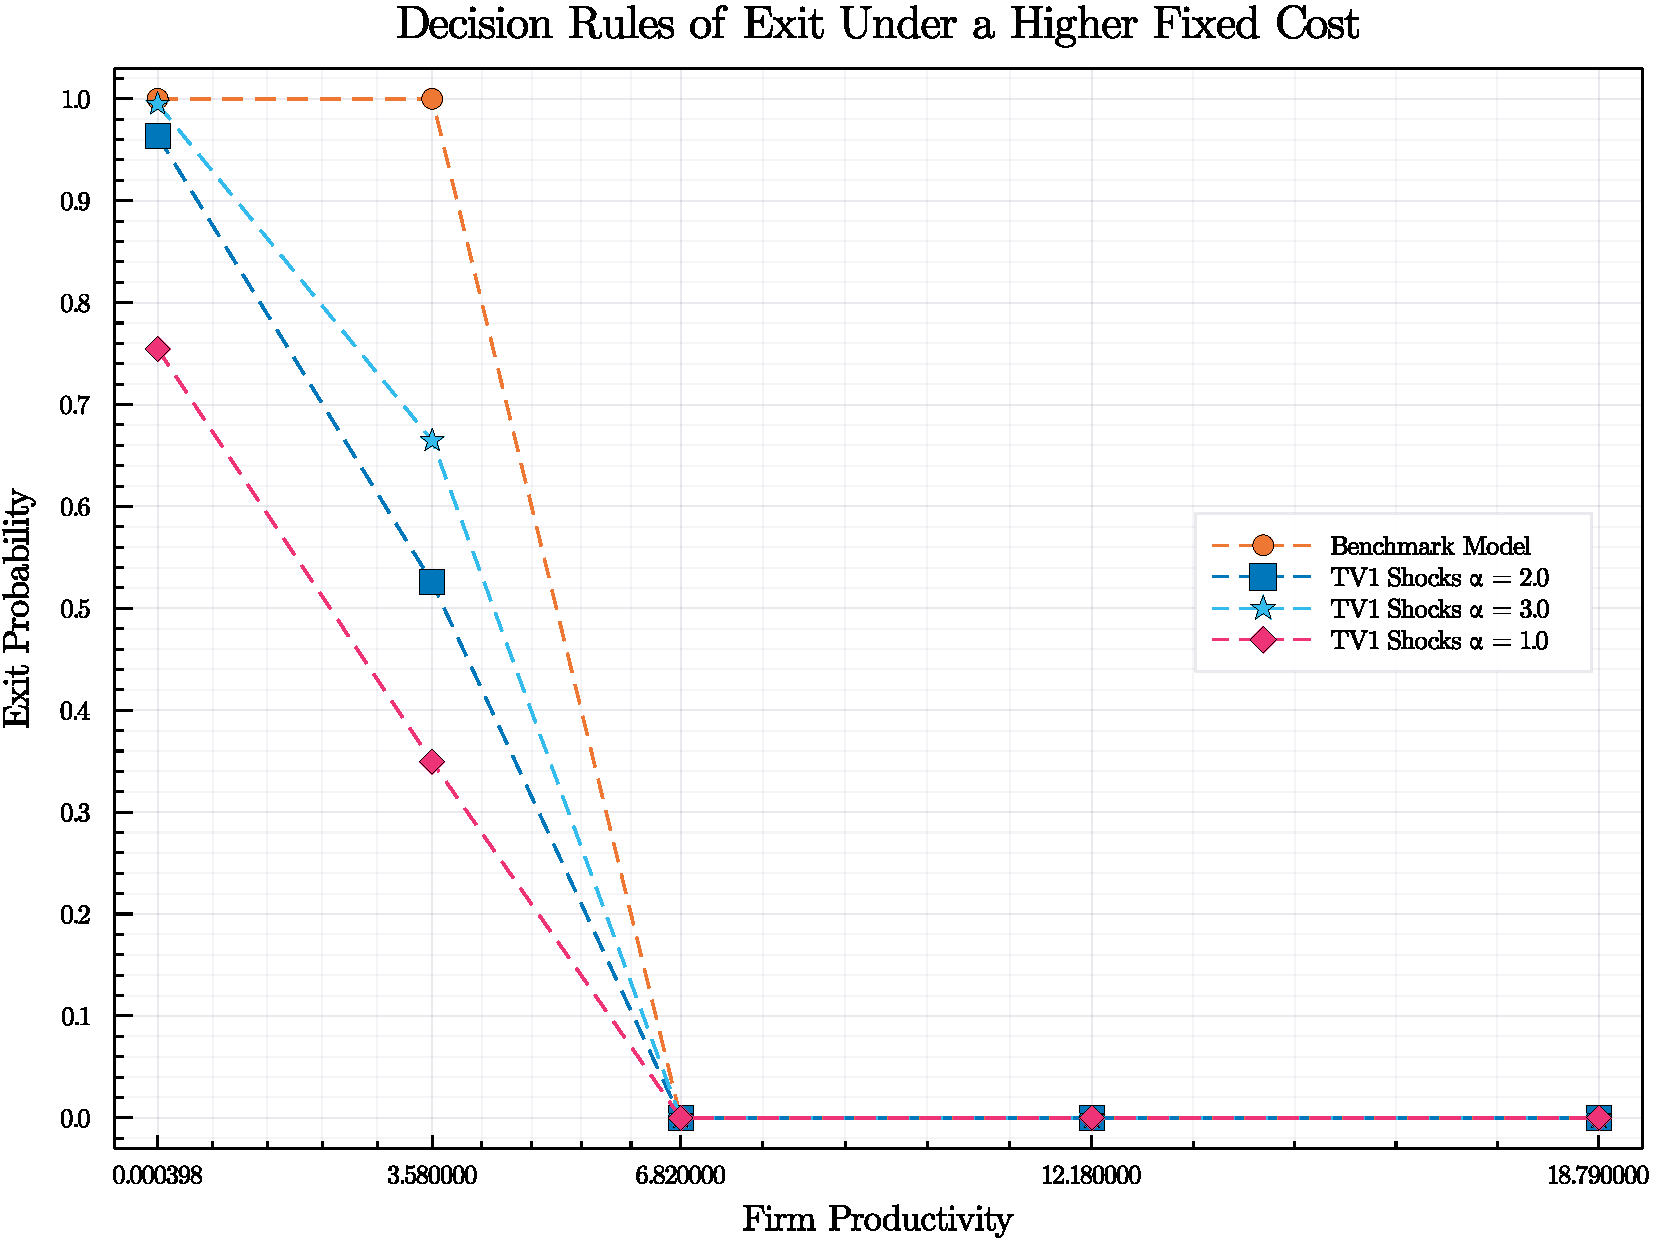
\includegraphics[scale=.35]{Figures/decision_rules_cf15.pdf}
	\caption{Decision Rules across Model Specifications when $c_{f}=15$ rather than $10$}
	\label{T4}
	\end{center}
\end{figure}
\end{solution}

\newpage
	\section*{Appendix}
 	The first code file runs the code.
 	\jlinputlisting{Code/run_model.jl}
	
 	The second code file contains the relevant functions.
 	\jlinputlisting{Code/hopenhayn_rogerson.jl}

\end{document}